\documentclass{article}

\usepackage{mathtools,amsfonts}
\usepackage{enumitem}
\usepackage{fullpage}
\usepackage{fancyvrb}
\usepackage{hyperref}


\begin{document}
\thispagestyle{empty}

\begin{center}
  \textbf{\Large Intermediate Test 1}
  % LEVEL is Senior, Intermediate or Beginner
  % NUMBER is the test number: 1, 2, etc.
  \\ \vspace{1em}
  \textbf{\large Stellenbosch Camp 2022}
  \\ \vspace{1em}
  \textbf{\large Time: $2\frac{1}{2}$ hours}
\end{center}

\bigskip

\begin{enumerate}[itemsep=\fill]

\item % Tim, 2022
Ian is placing $3$ $\mathbf{L}$-shaped tiles and a single square tile on a $2\times5$ chessboard. How many ways can Ian tile this board by placing all the tiles such that no tiles overlap and all squares are covered?
\begin{center}
    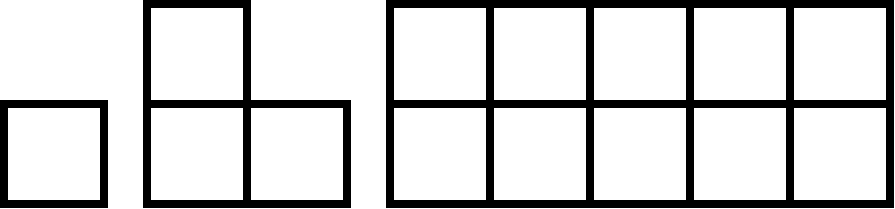
\includegraphics[scale=0.3]{intermediate_Q1_shapes.png}
\end{center}


\item % Tim, 2022
Given a triangle $ABC$, with $AB = BC = 1$, what is the maximal area that can be achieved by varying the length of the third side $CA$?

\item % Andrew, 2022
Given an acute angled triangle with sides of lengths $a,b$ and $c$. Prove that: \[a^2 + b^2 > c^2\]

\item % Liam, 2022
Where $p$ is a prime and $n\in\mathbb{N}$, find all solutions to the equation \[p^2 = 2^n + 1.\]

\vspace{0pt}

\item % Tim, 2022
There are at least 3 people at a party. All of them have an even number of friends, where friendship is mutual. Show that there are 3 of them who each have the same number of friends.

\end{enumerate}


\vfill
% ASCII art
\centering
\small
\begin{BVerbatim}
% Insert art here
\end{BVerbatim}

\end{document}
